\let\textcircled=\pgftextcircled


\chapter{Background}
\label{chap:background}

The idea of autonomous vehicles(AVs) is not new. As early as 2005, DARPA had invested heavily in the creation of unmanned trucks and organised for the Urban Challenge \cite{buehler2009darpa} to allow for different teams to showcase their unmanned vehicles. However, due to the challenges such as low computational power and underdeveloped AI and ML systems, the resulting implementations were not practical and had a high fault rate of 1 fault in 100 miles compared to the human fault rate of around 1 in 100 million miles. Nonetheless, from this challenge, it was clear that the prospect of AVs was plausible and indeed possible. 

Currently, AVs are divided into five levels of autonomy as defined be the Society of Automotive Engineers(SAE):
\begin{table}[H]
	\begin{tabular}{p{1cm}p{\linewidth}}
		\textbf{SAE level} & \textbf{Description}                                                                                                                                         \\ \hline
		\textbf{0}         & No AV control systems. An example is blind spot indicators.                                                                                                  \\
		\textbf{1}         & Basic driver assistance built into vehicle design. An example is the cruise control function.                                                                \\
		\textbf{2}         & Basic AV control systems. Driver required to monitor the environment and take back control if need be. A good example is the Tesla Autpilot.                 \\
		\textbf{3}         & AVs can safely navigate and drive within mapped environment. Driver required to monitor the environment and take back control if need be.                    \\
		\textbf{4}         & Highly autonomous control capable of handling most conditions but the driver has the option to take control. Renault ISymbioz is an example of a level 4 AV. \\
		\textbf{5}         & Completely autonomous with zero human involvment.                                                                                                           
	\end{tabular}
\end{table}


%The race to level 5 autonomous by different companies has seen major competition between these industry players. As such, they have invested heavily in designing and deploying AVs. However, these vehicles tend to have various sensors as seen in figure \ref{fig:my_label}. These sensors are necessary for accurate navigation and safety. Nonetheless, they are quite expensive thereby making AVs not feasible at the moment. 

\section{Components of an AV}

\begin{itemize}
	\item \textbf{LiDAR} - LiDAR provides highly detailed 3D information about the environment around the vehicle and objects in it. LiDAR operates by sending out pulses of lasers and recording the reflections of the pulses from objects. By comparing this with the time taken for the lasers to be reflected(time of flight) and their direction, the distance of these objects can be calculated and mapped in a point cloud. 

	LiDAR units require complex optical systems that are expensive to build. As a result,  they are the most expensive sensors in AVs with the top end such as Velodyne HDL-64E shown in figure \ref{fig:lidar} costing more than 50,000\$. 
	In a bid to reduce the cost of LiDAR units,  different companies are exploring different design methods that are cheaper but still able to offer the same performance as the top end LiDAR units such as solid state LiDAR\footnote{See appendix \ref{app:lidar}}.
	
	 \begin{figure}[h]
	 	\centering
	 	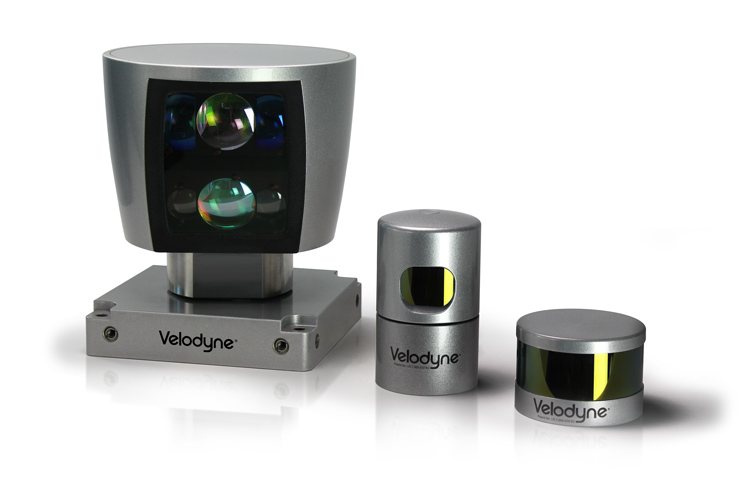
\includegraphics[width=\textwidth]{media/hdl-family.png}
	 	\caption{Velodyne LiDAR family. From left: Velodyne HDL-64E , HDL-32E , VLP-16}
	 	\label{fig:lidar}
	 \end{figure}
	
	\item \textbf{Cameras} - Cameras mounted on the vehicle are used for classification and identification of various objects on the road. 
	Cameras can also be used to create 3D maps of the surrounding environment.By combining two cameras, a stereo image can be captured that provides depth information. Alternatively, by combining a camera and IR Laser sensor for depth estimation, RGB-D \cite{henry2010rgb} images are obtained and mapped in a point cloud.
	
	\item \textbf{Position Estimators} - Position estimators are a group of sensors used for navigation of the vehicle. These include GPS systems, odometers and gryometers. 
	\item \textbf{Distance Sensors} - Distance sensors such as radars and sonars are important for gauging the distance of objects on the road. 
	Radars are the most commonly used distance sensors and they work by transmitting radio waves and recording the reflected radio waves from objects. As compared to cameras and LiDARs, radars work well in a variety of low visibility scenarios such as poor weather. 
	However, the reflectivity of these radio waves depends on the nature of objects, their size, absorbtion characteristics and the transmitting power. As such, it is may not be effective for detecting objects with low absorbtion characteristics such as pedestrians and animals.
	
	\item \textbf{Processing Unit} - In order to process all the data from sensors on the vehicle, AVs require powerful processing units to to do so in real time. Most ML/AI algorithms used for detecting and identifying objects from LiDAR and camera data demand large amounts of processing power. This is achieved through the use of CPUs, GPUs, Field Programmable Gate Arrays(FPGA)\cite{brown2012field}, Application Specific Integrated Circuits(ASICs)\cite{smith1997application} or combinations with each other. 

\end{itemize}


\begin{figure}[t]
	\centering
	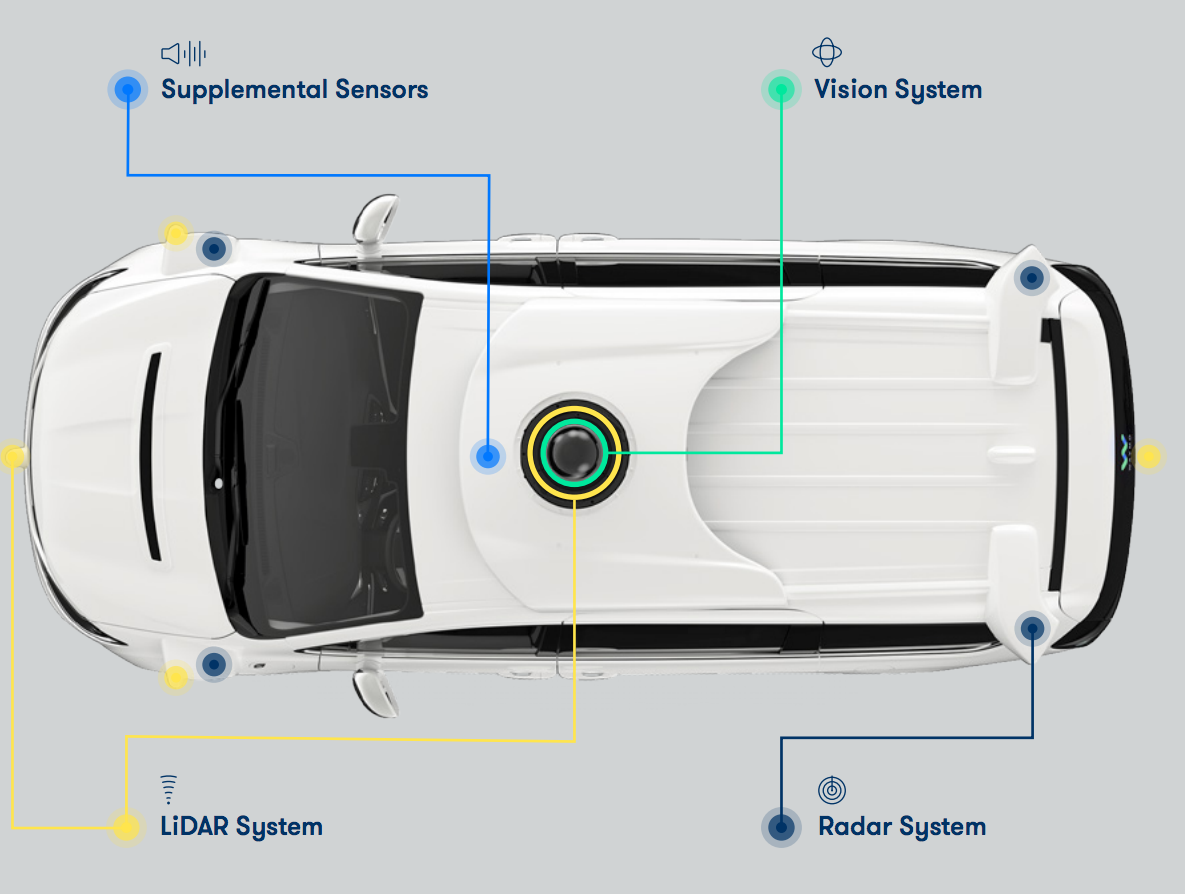
\includegraphics[width=\textwidth]{media/waymo.png}
	\caption{Components of Waymo's Self Driving Car, Source:\cite{waymo_2018}}
	\label{fig:my_label}
\end{figure}


AVs have three main modes of operation namely,
\begin{itemize}
	\item \textbf{Perception} - This is the first step which involves processing the input from the sensors. In this mode tasks such as object detection and tracking, lane detection, traffic sign detection and recognition are performed.
	\item \textbf{Planning} - This is the next step after detection and recognition tasks are performed . In this stage route and trajectory planning algorithms are run  to plan how the vehicle should navigate in the immediate environment as well as a route to a target location. These algorithms are required to handle complex situations to ensure safety of the passengers and other road users. 
	\item \textbf{Control} - This stage involves the execution of plans created in the planning stage. This stage is crucial as the actuators involved in steering and movement have to be able to be able to accurately follow the plans. This involves calculation of energy and forces. At this stage the trajectories and movement of other road users and objects have to be calculated in order to anticipate and avoid any accidents. 
	
\end{itemize}



\section{Industrial Approaches}
In order to be viable, AVs need to meet a few constraints as discussed in \cite{lin2018architectural}.
\begin{itemize}
	\item \textbf{Performance} \\
	At the moment there are no clear regulations as to how fast the perception, planning and control pipeline should be. However according to research by Brown et al. \cite{brown1994human}, humans take around 600 ms to respond and brake when expecting an interruption, however this figure shoots to 850 ms when an unexpected situation arises. In addition, Newell et al \cite{newell1985prospects}, established that the fastest human response time is between 100-150ms. These figures can be used as a baseline while developing a pipeline. In this pipeline, there are two factors to consider, namely the frame rate (frequency of the data from sensors) and the processing latency (time taken to process data). As such, an AV system should be able to react within 100ms, that is, faster than the human response time.
	
	\item \textbf{Storage} \\ 
	AVs should be able to store maps of different areas with fine granularity for accuracy during localisation. As a result, the storage of these maps can run into tens of Terabytes. Despite recent advances in cloud technology and the emergence of 5G connectivity that is significantly fast. Downloading these maps would take significant time and would also render the car unusable in case of no internet connectivity. As such, the vehicles should have enough storage to store these maps locally. 
	
	\item \textbf{Power} \\
	Most of the major industry players have moved to electric-vehicles for their AV systems. Depending on the equipment and sensor configurations used in these systems, the power usage can range from 500 watts to 1.5 kilowatts. Given that the AVs have limited battery capacity, heavy power consumption by these systems can lead to poor driving ranges hence making the cars less viable. As such the configuration of these systems has to be carefully considered to ensure a reasonable driving range. 

	\item \textbf{Thermal} \\
	Processing components in the AV systems such as CPUs and GPUs require a significant amount of energy to cool. This is necessary to ensure that they operate within their recommended thermal operating range. Failure to do so could result in the failure of these systems. As such, additional cooling systems have to be installed in the vehicle in order to ensure this.
	
\end{itemize}
Following the discussion above, the next subsections will review how different industry players are implementing their AV systems with special focus to the issue of perception
\begin{figure}
	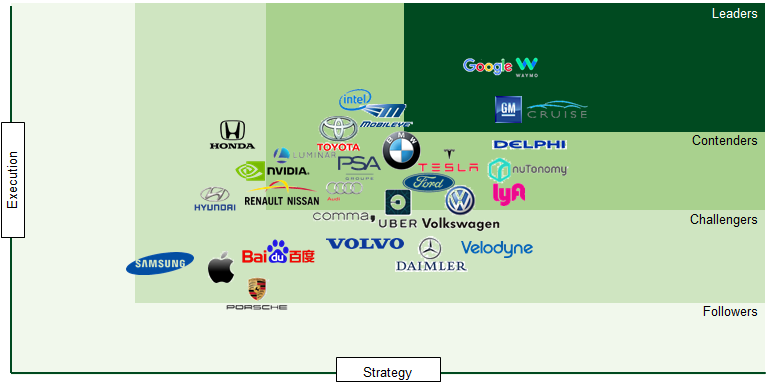
\includegraphics[width=\textwidth]{media/avind.png}
	\caption{AV Leaderboard. Navigant Research. Source:\cite{navigantresearch_2018}}
\end{figure}
\subsection{Camera}
Mobileye\cite{mobileye_2018}, is one of the top contenders in the development of camera only AVs. It was recently acquired by Intel and believes that AVs should be able to accurately and safely navigate using cameras only given the fact that humans are able to do so with vision only. Previously, MobilEye was a supplier of vision systems for Advanced Driver Assistance Systems and had a partnership with Tesla to supply their vision systems prior being acquired by Intel. 
Given their extensive background in developing these vision systems, the partnership with Intel aims to develop a complete autonomous driving package.\cite{intelsolutions_2018}
 

\subsection{Camera and  Radar}
Another major contender that is using the camera and radar configuration is Tesla. Elon Musk, the founder, believes that LiDAR is not necessary for AV perception following a similar argument as MobilEye. However, this argument was dispelled following a recent crash whereby due to bright sunlight, a Tesla vehicle on 'autopilot' mode was unable to detect a white vehicle thus resulting into an accident leading to loss of life. The invariance of LiDAR to different lighting conditions could have helped in detecting the vehicle. 

\subsection{LiDAR, Camera and Radar}
This configuration is used by most of the leading industry players such as Uber, Waymo and GM Cruise. This configuration has proven to be robust and accurate. However, in order to process the amount of fused data, they require large amounts of computational power which in turn may lead to increased power usage. 


\section{Object  Detection} 
In this section, related research on object detection methods for AV perception will be discussed. 




\subsection{Object Detection using Classic Computer Vision Methods}
Classic computer vision methods have advanced over the years from simple algorithms such as SIFT\cite{lowe1999object} and SURF\cite{bay2006surf} which use descriptors to detect interesting points in images for object detection to much higher level representations such as the Histogram of Gradient(HOG)\cite{dalal2005histograms} or Haar Features\cite{viola2001rapid}  that were used in classifiers.  However, these methods have been unreliably slow and not as accurate. In addition these features are only able to model 2D data. 3D methods such as Intrinsic Shape Signatures(ISS)\cite{}, NARF\cite{} and Uniform Sampling have since been developed but are lacking in terms speed. Furthermore, these feature detectors have to be hand-crafted manually which is a tedious process. As a result, they are rarely used in real-time AV applications due to their speed and accuracy.


\subsection{Object Detection using Deep Learning}
The advancement of neural networks has offset the reliance of classical methods of object detection by allowing for features to be automatically learnt by the network without the need for manual feature extraction. This is attributed to the networks having numerous number of deep layers that are able to capture these features.  
\subsubsection*{Convolutional Neural Networks(CNN)}
The idea of CNNs has been there for over two decades now and are inspired by the idea of receptive fields in the primary visual cortex. Currently, they are widely used in image object detection tasks and various CNN architectures have been developed. As compared to regular neural networks which have all neurals connected to each other between hidden layers, neurons in CNNs are connected to a small region in the layer before it(receptive field) and have three dimensions(width,height and depth). By doing so this reduces the number of parameters to be tuned during backpropagation as well as stored. 
\begin{figure}[h]
	\centering 
	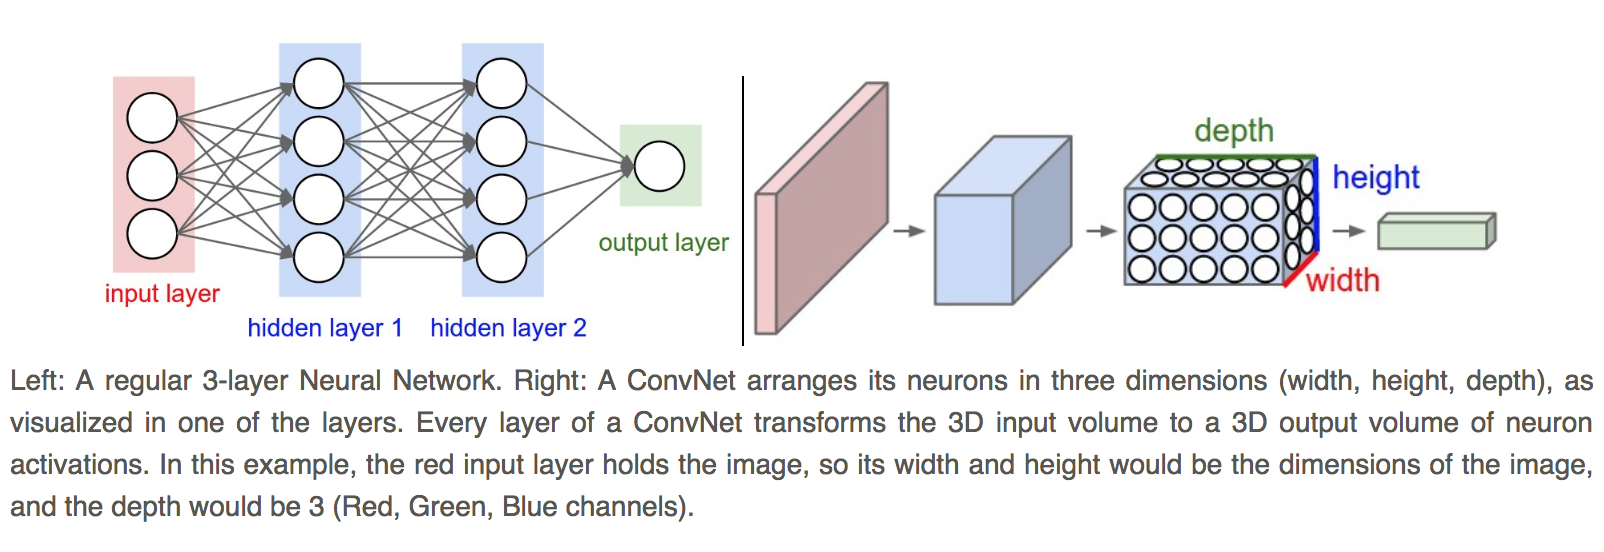
\includegraphics[width=\linewidth]{images/neuralnet}
	\caption{NN vs CNN Source:\url{https://cs231n.github.io/convolutional-networks}}
	\label{fig:cnn}
\end{figure}


Most architectures consist of five main layers:
\begin{itemize}[noitemsep]
	\item  \textbf{Input Layer} Raw image data is fed through this layer. 
	\item  \textbf{Convolution Layer} This layer calculates the output of neurons connected to a receptive field.
	The size of the output is determined by the following equation. 
	
	$A_{out}= (A_{in}-K+2P)/S+1$
	
	where $A_{in}$ is the input size,  $A_{out}$ is the output size, K is the kernel size, P is the padding size and S is the stride of the kernel. 
	\item  \textbf{Activation Layer} In this layer the output of the convolution is passed through an activation function such as sigmoid, ReLU or TanH. 
	\item  \textbf{Pooling Layer} This layer downsamples the  output of the activation layer along the width and height dimensions. 
	\item \textbf{Fully connected layer} Finally, this layer computes the probability scores for different classes by connecting all neurons from the pooling layer. 
\end{itemize}

\subsubsection*{Region Proposal Networks(RPN)}
R- CNN\cite{} brought forth the idea of region based CNNs with the aim of increasing the accuracy of CNNs. By using selective search, regions of interest(ROI) in input images are proposed. These regions are then resized are then fed through a CNN to generate a bounding box and classification of the image. Finally a classifier, regressor are run on the output. However as this method requires a forward pass of the CNN for each proposal, its speed was quite slow. It also required the CNN, classifier and regressor to be trained separately. 
Fast R-CNN\cite{girshickICCV15fastrcnn} iterated on R-CNN to further improve the speed and accuracy by using ROIPooling whereby instead of running each proposal in a CNN, regions that were overlapping were pooled and fed through the cnn thus sharing the computation. Furthermore, this model was end to end and thus combined the  classifier and regressor  by adding a softmax layer and linear regression layer after the CNN.
Faster R-CNN\cite{ren2015faster} sought to remove the bottleneck imposed by the using selective search to propose regions. By using a sliding window with various anchor boxes on features maps generated by a forward pass of a CNN, bounding boxes on certain regions of the image could be generated. These regions were then passed onto Fast R-CNN to classify the objects. 
\begin{figure}[h]
	\centering
	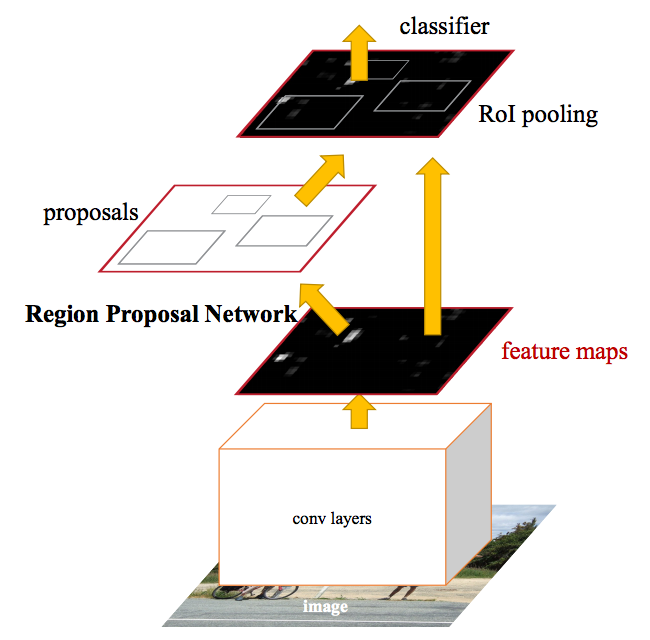
\includegraphics[width=0.5\linewidth]{images/fastercnn}
	\caption{Faster R-CNN overview. Source:\cite{ren2015faster}}
\end{figure}


Depending on the input, these two network architectures have formed the back bone of most 2D and 3D object detection applications. 
\paragraph{Monocular Vision} 
Monocular vision is derived from a single camera. This representation is 2D and lacks depth information. Mono3D by Chen et al \cite{chen2016monocular} is a state of the art object detection model that uses monocular images where they were fed through a CNN and the resulting 2D object proposals were extruded into 3D bounding boxes by performing segmentation.

\paragraph{Stereo Vision}Stereo vision involves calibrating two cameras intrinsically and extrinsically by matching similar points in images from both cameras. Using the resulting stereo image, it is possible to estimate the depth of objects in the image. However the accuracy of this depends on a few factors such as the resolution, camera quality, lens distortion and the calibration algorithm. 3DOP \cite{chen20183d} is one of the state-of-the-art models that use stereo images in CNNs to detect objects.  

\paragraph{LiDAR+Camera}
By fusing input from a monocular image and point clouds, it is possible to extract depth information from the images. Chen et al further reiterated their monocular approach into MV3D\cite{chen2017multi} a multiview 3D object detection network. In their work, they were able to fuse LiDAR and camera input to create a bird's eye view of the surrounding environment and further perform object detection of features. 


\paragraph{LiDAR} 
Point cloud object detection is particularly challenging as established 3D object detection methods for images cannot be applied to point clouds. Point clouds are a set of geometric points in a euclidean space. They are unordered in nature and this presents a particular problem to deep learning methods as they need to be invariant to permutations of the input set.
Depending on how they manipulate the point clouds, current point cloud based object detection models can be split into three groups:
\begin{enumerate}
	\item \textbf{Direct Manipulation} \\ . 
	Pointnet\cite{qi2017pointnet} developed by Qi et al was able to overcome this challenge on small sets of point clouds. By using point clouds as direct input into Recurrent Neural Networks\cite{medsker2001recurrent} They were able to create a global point cloud signature that could classify and segment 3D objects in the point cloud. They further improved this model into Pointnet++\cite{qi2017pointnet++} which recursively applied PointNet on nested partitions of the point clouds using a hierarchical neural network. In doing so they were able to capture the local structures of the point clouds as a result of their metric nature and thus achieve better performance than PointNet. However this approach has high memory and computational requirements. For both of these publications, the source code was released for public use. Consequently, they have formed a fundamental foundation for further development of point cloud object detection methods such as F-PointNet\cite{qi2017frustum}.
	
	\item \textbf{Voxel Based} \\
	By dividing the pointclouds into 3D voxel grids, points within these voxels can be sampled to perform feature extraction. VoxelNet \cite{zhou2017voxelnet} is a state of the art architecture that uses this method to extract these features through Voxel Feature Extraction layer. The extracted features are then fed through a RPN to generate bounding boxes and classify objects within them. 
	
	\item \textbf{2D-Based }\\
	This involves projecting the pointcloud into a 2D image plane coordinate system which can then be trained on existing image based CNNs  such as VGG-16. VeloFCN \cite{li2016vehicle} was one of the first methods to implement this approach using a fully convolutional network. However, VeloFCN lacked bird eye and front view representations. 
	
\end{enumerate}



\begin{table}[h]
	\centering
	\begin{tabular}{|l|l|l|l|}
		\hline
		\textbf{Network Model} & \textbf{Mode}         & \textbf{Code} & \textbf{Inference Time}  \\ \hline
		\textbf{VoxelNet}      & \textit{LiDAR}        & Unnoficial    & \textit{\textbf{100ms}} \\ \hline
		\textbf{AVOD}          & \textit{LiDAR+Image}  & Yes           & \textit{\textbf{100ms}} \\ \hline
		\textbf{MV3D}          & \textit{LiDAR+Image}  & Unnoficial    & 360ms                   \\ \hline
		\textbf{MONO3D}        & \textit{Mono Image}   & Yes           & 4.2s                    \\ \hline
		\textbf{3DOP}          & \textit{Stereo Image} & Yes           & 3s                      \\ \hline
	\end{tabular}
	\caption{Modes of Operation of Common Architectures}
	\label{tab:arch}
\end{table}







\section{Legal, Ethical and Economic Considerations}


Despite improvements in traffic safety over the years, over  2.2$\%$ of deaths globally are caused by road accidents. Of these accidents, 94$\%$ are as a result of human error. It has been argued that AVs will reduce this figure by 

According to \cite{gasser2016fundamental}, there are no public laws that cover the  use of independent autonomous vehicles in public spaces. In his article, he cites the fundamental issue as "understanding and accepting the effect of AVs as an independent action by a machine". Due to the lack of public laws on their use, he proposes extending fundamental rights such as the right to life into the framework for creating laws that cover emerging technologies that have an effect on the public, that are otherwise not accounted for in traditional laws.

 
Bearing this in mind, it is important to note that  It has been predicted that upon mainstream 

This creates a realistic baseline that can then be extended in evaluating the performance of AV systems. As such, if the risk of automation is lesser than the risk of human vehicle control then the AV would be beneficial. Consequently, the AVs are not to be considered as perfect systems but instead should be treated as systems that minimise the overall risk to the passenger and also their surroundings. 



%
%
%
%The classic ethical dilemma for self driving cars poses a scenario whereby AVs are presented with a situation whereby a fatal accident is inevitable. For example, the AV either has to crash into a group of people in order to save the life of a passenger or to crash itself and sacrifice the life of the passenger. This dilemma highlights important legal, ethical and economic considerations to be considered by companies involved in the production of AVs and their corresponding systems. 
%
%
%According to \cite{gasser2016fundamental}, there are no public laws that cover the  use of independent autonomous vehicles in public spaces. In his article, he cites the fundamental issue as "understanding and accepting the effect of AVs as an independent action by a machine". Due to the lack of public laws on their use, he proposes extending fundamental rights such as the right to life into the framework for creating laws that cover emerging technologies that have an effect on the public, that are otherwise not accounted for in traditional laws. 
%
%Bearing this in mind, it is important to note that despite improvements in traffic safety over the years, 94\% are still caused by human beings with a large majority of them being fatal with the current human error rate being 1 in 100 million miles. This creates a realistic baseline that can then be extended in evaluating the performance of AV systems. As such, if the risk of automation is lesser than the risk of human vehicle control then the AV would be beneficial. Consequently, the AVs are not to be considered as perfect systems.
%
%With regard to economic considerations, car manufacturers involved in the production of AVs have to ensure that their AVs are able to handle numerous scenarios even if they are rare or considered statistically impossible. They should also be required to take legal liability in case any of their system components are defective and result in failures or accidents. This is important for customer trust without which they will not be able to convince customers to shift to AVs. In addition, for the adoption of AVs to be widespread, they have to be reasonably priced and efficient. With the current prices of the the various components and their power consumption, the adoption of AVs at the moment is not viable. 
%
